\chapter{Black-Scholes Model}
\label{ch:BS}

\section{Black-Scholes Model}
Suppose that stock price $S$ follows a geometric Brownian motion

\begin{equation}
dS = \mu Sdt + \sigma SdW
\label{eq:bs_gbm}
\end{equation}

we are going to derive a partial differential equation (PDE) for the price of a derivative based on such a stock.

The model proposed by Black and Scholes relies on the following set of additional assumptions (besides the geometric Brownian motion):
\begin{itemize}
\tightlist 
\item constant risk-less interest rate $r$;
\item no transaction costs;
\item it is possible to buy/sell any (also fractional) number of stocks; similarly with the cash;
\item no restrictions on short selling;
\item option is of European type.
\end{itemize}

After the derivation of the model equation we will determine the explicit solution for European call and put options.

\subsection{Merton Derivation}
In this Section we are going to provide the steps followed by Merton to derive the Black-Scholes PDE.

Firstly, let's consider the case of a non-dividend paying stock. Imagine a portfolio consisting of options, stocks and cash with the properties that at each time $t$ the portfolio has zero value and it is \emph{self-financing}, which means that if there is no exogenous infusion or withdrawal of money, the purchase of a new asset must be financed by the sale of an old one.

Let be 
\begin{itemize}
\item $Q_S$, the number of stoks, each of them with value $S$;
\item $Q_V$, number of options, each of them with value $V$;
\item $B$, cash on the account, which is continuously compounded using the risk-free rate $r$.
\end{itemize}

The required properties can be formulated mathematically as
\begin{equation}
\begin{cases}
SQ_S+VQ_V+B=0 \\
SdQ_S + V dQ_V +\delta B = 0 \\
dB = rBdt+\delta B
\end{cases}
\label{eq:bs_properties}
\end{equation}

Differentiating the first of Eq.~\ref{eq:bs_properties}
\begin{equation}
\begin{split}
&d(SQ_S + VQ_V +B) = d(SQ_S + VQ_V) + \overbrace{dB}^{rBdt+\delta B} = 0 \\
& \overbrace{SdQ_s + VdQ_V +\delta B}^{=0} + Q_S dS + Q_V dV + rBdt = 0 \\
& Q_SdS+Q_VdV \overbrace{-r(SQ_S + VQ_V)}^{rB}dt=0\\
\end{split} 
\end{equation}
Dividing by $Q_V$ and setting $\Delta = -\frac{Q_S}{Q_V}$
\begin{equation}
dV -rVdt-\Delta (dS - rSdt)=0
\end{equation}
$dS$ can be determined from Eq.~\ref{eq:bs_gbm}, while $dV$ applying It$\hat{o}$'s lemma. Then we choose $\Delta$ (i.e. the ratio between the number of stocks and options) so that it eliminates the randomness (i.e. the coefficient at $dW$ is zero).
  
\begin{equation}
dV = \left(\cfrac{\partial V}{\partial t} + \mu S  \cfrac{\partial V}{\partial S} + \cfrac{1}{2} \sigma^2 S^2  \cfrac{\partial^2 V}{\partial S^2} \right) dt + \sigma S \cfrac{\partial V}{\partial S} dW
\end{equation} 
Therefore:
\begin{equation}
dP =  \left(\cfrac{\partial V}{\partial t} + \mu S  \cfrac{\partial V}{\partial S} + \cfrac{1}{2} \sigma^2 S^2  \cfrac{\partial^2 V}{\partial S^2} + \delta \mu S\right) dt + \left(\sigma S  \cfrac{\partial V}{\partial S} + \delta \sigma S \right)dW
\end{equation}
We eliminate the randomness
\begin{equation}
\delta = -\cfrac{\partial V}{\partial S}
\end{equation}

\begin{equation}
\cfrac{\partial V}{\partial t} + \cfrac{1}{2} \sigma^2 S^2 \cfrac{\partial^2 V}{\partial S^2}+ rS \cfrac{\partial V}{\partial S} − rV = 0
\end{equation}

\section{Solutions of Black-Scholes PDE}
Now we need to find a solution $V(S, t)$ to the partial differential equation which holds for $S >0$, $t \in [0, T)$.

So far we have not used the fact that we consider an option (in general the PDE holds for any derivative that pays a payoff at time $T$ depending on the stock price at this time).
Clearly the type of derivative determines the terminal condition at time $T$, so in general $V(S, T)$ = payoff of the derivative.

\subsection{Simple Solutions}
How to price the derivatives with the following payoffs:
\begin{itemize}
\tightlist
\item $V(S, T) = S$, it is in fact a stock so $V(S, t) = S$
\item $V(S, T) = E$ with a certainty we obtain the cash $E$ ($V(S, t) = Ee^{−r(T−t)}$)
\end{itemize}
by substitution into the PDE it is possible to check that they are indeed solutions.
%EXERCISES:
%Find the price of a derivative with payoff
%$V(S, T) =S^n$,where $n\in N$.

%HINT: Look for the solution in the form
%$V(S, t) =A(t)S^n$

%Find all solutions to the Black-Scholes PDE, which are independent of time, i.e., for which
%$V(S, t) = V(S)$

\subsection{Binary Options}
Let us consider a binary option, which pays \$1 if the stock price is higher that $K$ at expiration time, otherwise its payoff is zero.
In this case
\begin{equation}
V(S, T) = 
	\begin{cases}
		1, \quad\textrm{if }S > K\\
		0, \quad\textrm{otherwise}	
	\end{cases}
\end{equation}

This partial differential equation (PDE) can be solved directly with numerical methods. But then some tricky stability issues must be tackled. Here we prefer applying variable transformations as much as possible in order to obtain simpler equation form (i.e. the goal is to re-formulate Black-Scholes PDE into a heat equation).

The first step is to apply the transformation $x = \textrm{ln}(S/K)$ and a new function $Z(x, \tau) = V (Ee^x, T -\tau)$. 
The PDE for $Z(x, \tau)$ becomes:
\begin{equation}
\begin{gathered}
\cfrac{\partial Z}{\partial \tau} -\cfrac{1}{2}\sigma^2 \cfrac{\partial^2 Z}{\partial x^2}+\left(\cfrac{\sigma^2}{2}−r\right)  \cfrac{\partial Z}{\partial x} + rZ = 0\\ \\
Z(x, 0) =V(Ee^x, T)
\end{gathered}
\end{equation}

Then we want the PDE to become a heat equation. This is done by considering the new function $u(x,\tau)=e^{\alpha x + \beta\tau}Z(x,\tau)$ where the constant $\alpha, \beta \in \mathbb{R}$ are chosen so that the PDE for $u$ is the heat equation.

The corresponding PDE for $u$ is
\begin{equation}
\begin{gathered}
\cfrac{\partial u}{\partial \tau} -\cfrac{\sigma^2}{2} \cfrac{\partial^2 u}{\partial x^2}+A\cfrac{\partial u}{\partial x} + Bu = 0\\ \\
u(x,0)=e^{\alpha x}Z(x,0)=e^{\alpha x}V(Ke^x, T)
\end{gathered}
\end{equation}
where
\begin{equation}
\begin{cases}
A=\alpha\sigma^2 + \cfrac{\sigma^2}{2}-r\\
B=(1+\alpha)r-\beta-\cfrac{\alpha^2\sigma^2+\alpha\sigma^2}{2}
\end{cases}
\end{equation}

In order to have $A=B=0$ to get the heat equation we set
\begin{equation}
\begin{cases}
\alpha=\cfrac{r}{\sigma^2}-\cfrac{1}{2}\\
\beta=\cfrac{r}{2}+\cfrac{\sigma^2}{8}+\cfrac{r^2}{2\sigma^2}
\end{cases}
\end{equation}

The solution $u(x,\tau)$ of the resulting PDE is given by hte \emph{Green formula}
\begin{equation}
u(x, \tau)=\cfrac{1}{\sqrt{2\sigma^2\pi\tau}}\int^{+\infty}_{-\infty}e^{-\frac{(x-s)^2}{2\sigma^2\tau}}u(s,0)ds
\end{equation}

After evaluating the integration it is possible to find the original solution $V(S,t)$ performing backward substitutions

\begin{equation}
V(S, t) = e^{-r(T-t)}N(d_2)
\end{equation}
where $d_2=\frac{\textrm{log}(\frac{S}{K}+\left(r-\frac{\sigma^2}{2}\right)(T-t)}{\sigma\sqrt{T-t}}$.

\subsection{Call Option}
In this case
\begin{equation}
V(S,T)=\textrm{max}(0,S-K)=
\begin{cases}
S-K,\quad \textrm{if}~S>K\\
0, \quad\textrm{otherwise}
\end{cases}
\end{equation}

The steps are similar to the previous example (i.e. same sequence of transformations, initial conditions for the heat equation):
\begin{equation}
u(x,0)=
\begin{cases}
e^{\alpha x}(S-K),\quad \textrm{if}~x>0\\
0, \quad\textrm{otherwise}
\end{cases}
\end{equation}
and similar evaluation of the integral.

Finally the option price
\begin{equation}
V(S,t) = SN(d_1)-Ke^{-r(T-t)}N(d_2)
\end{equation}
where $N$ is the distribution function of a normalized normal distribution and  $d_1=\frac{\textrm{log}(\frac{S}{K}+\left(r+\frac{\sigma^2}{2}\right)(T-t)}{\sigma\sqrt{T-t}},\quad d_2=d_1-\sigma\sqrt{T-t}$.

Figure~\ref{fig:call_option} shows the option price as a function of the stock price for various values of $t$.

\begin{figure}[htb]
	\centering
	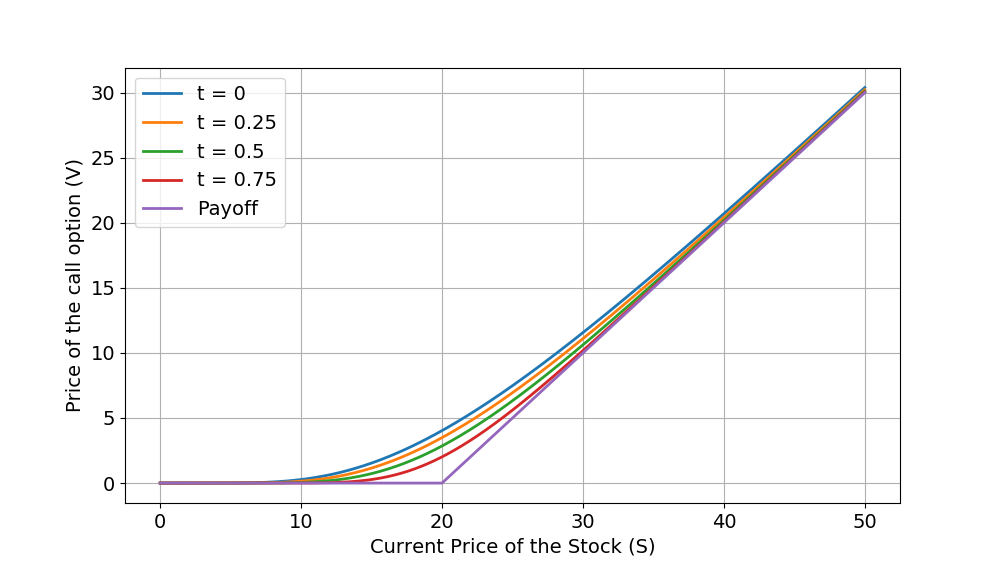
\includegraphics[width=0.9\textwidth]{figures/call_option_price}
	\caption{Option price as a function of the underlying price for various values of $t$.}
	\label{fig:call_option}
\end{figure} 

\section{Risk Neutral Valuation}
Risk neutral valuation concept arise from one of the key properties of the Black-Scholes differential equation: it does not involve any variable that is affected by the risk preference of the investor. 
The variables that appear in the eqaution are indeed: the current stock price, the stock price volatility, time and the risk-free rate of interest. All of them are independent of risk preference.

This would not be true if the BS-PDE involved the expected return ($\mu$) on the stock. In fact $\mu$ depends on the risk preferencies: the higher the level of risk aversion by investors, the higher the return will be for any given stock.

Because BS differential equation is independent on risk its solutions must be unaffected by $\mu$, hence any set of risk preferences can be used in evaluating it. In particular, the very simple assumption that all investors are \emph{risk neutral} can be made.

In such a world, the expected return on all investments is the risk-free rate of interest ($r$). The reason is that risk-neutral investors do not require premium to induce them to take risks. It is also true that the present value of any cash-flow in a risk-neutral world an be obtained by discounting its expected value at the risk-free rate as well.

Then a derivative can be valued by using the following procedure:
\begin{enumerate}
\item assume that the expected return from the underlying asset is the risk-free interest rate $r$;
\item calculate the expected payoff from the derivative;
\item discount the expected payoff at the risk-free interest rate.
\end{enumerate}

Note that risk-neutral valuation is merely an artificial device for obtaining solutions to the Black-Scholes differential equation. Nevertheless the obtained solutions are valid in all worlds; moving from a risk-neutral world to a risk-averse world, two things happen. The expected growth rate in the stock price changes and the discount rate that must be used for any payoffs from the derivative changes. It happens that these two changes always offset each other exactly.

\section{Exercises}
\input{options_ex_text}

\begin{thebibliography}{9}
\end{thebibliography}
